\section{Komunikacja asynchroniczna w systemach rozproszonych -- Message Broker i architektura Message Bus}

\subsection{System rozproszony}

\par Systemem rozproszonym\english{Distributed System} nazywamy zbiór niezależnych komputerów, które tworzą jednolity system. Kluczowymi cechami są tutaj równoległość przetwarzania, współdzielenie zasobów, tolerancja na błędy, skalowalność oraz transparentność. Systemy te mogą być rozszerzane bez przerywania ich pracy (skalowane), są w stanie tolerować błędy oraz radzić sobie z awariami poszczególnych komponentów, w taki sposób, że działanie innych poszczególnych elementów, jak i całości systemu nie jest zagrożone. W ten sposób pozwalają ukryć złożoność większego rozwiązania i podzielić go na mniejsze problemy, rozwiązywalne poprzez poszczególne serwisy.

\begin{figure}
    \centering
    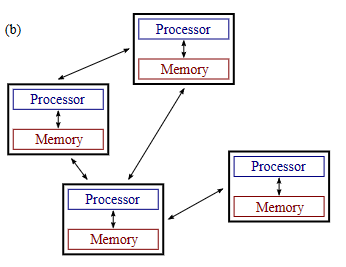
\includegraphics[width=\linewidth]{Distributed System - Wikipedia}
    \caption{System Rozproszony}
    \label{fig:distibutedSystemWikipedia}
    \source{Wikipedia}
\end{figure}

\par W takich systemach komunikacja odbywa się poprzez wymianę wiadomości. Pozwala to na realizację określonych celów. Proces ten może odbywać się z użyciem wielu metod, na przykład z wykorzystaniem protokołu \texttt{HTTP}. Innym rozwiązaniem pozwalającym na wymianę informacji jest wykorzystanie \emph{Message Broker}a.

\subsection{Message Broker i Service Bus}

\par \emph{Message Broker} jest oprogramowaniem, które pełni funkcję pośrednika w komunikacji pomiędzy poszczególnymi aplikacjami. Jest on centralnym punktem odpowiadającym za odbierania, a następnie przesyłanie wiadomości do stron zainteresowanych. Często znajdziemy tutaj rozwiązania, które zapewnią prawidłowe przekazywanie wiadomości według wybranej polityki, możliwość próby ponownego dostarczenia wiadomości, jak i możliwość stworzenia tak zwanej kolejki wiadomości martwych\english{Dead-letter Queue}.

\par Kluczowymi funkcjami \emph{Message Broker}a są:
\begin{itemize}
    \item \emph{Decoupling} - aplikacje komunikują się poprzez centralny punkt, którym jest \emph{Message Broker}, co pozwala im być niezależnymi od siebie. W systemie można dowolnie dodawać, jak i usuwać serwisy, bez negatywnego wpływu na pozostałe serwisy.
    \item \emph{Routing} - pozwala na kierowanie wiadomości na podstawie pewnych ustalonych cech, takich jak na przykład: temat, priorytet lub adresat.
    \item \emph{Reliability} - niezawodność poprzez zapewnienie gwarancji dostarczenia wiadomości, nawet pomimo tymczasowej niedostępności odbiorcy.
    \item Skalowalność\english{Scalability} - możliwość skalowania przepustowości poprzez dodanie kolejnych instancji \emph{Message Broker}a lub przez zastosowanie klastrów.
    \item Bezpieczeństwo - \emph{Message Broker} może oferować uwierzytelnianie i autoryzację, tylko dla klientów posiadających odpowiednie uprawnienia.
    \item Komunikacja asynchroniczna - umożliwia aplikacjom korzystającym z \emph{Message Broker}a dalszą pracę, bez konieczności oczekiwania na odpowiedź.
\end{itemize}

\par \emph{Service Bus} jest bardziej zaawansowanym rozwiązaniem, które oprócz funkcji \emph{Message Brokera} oferuje pełniejsze wsparcie dla transakcji i złożonych operacji. Wchodzi ono zazwyczaj w skład kompleksowych rozwiązań takich jak na przykład \emph{Enterprise Service Bus}. Zapewniają one nie tylko przesyłanie wiadomości, ale i ich koordynację i zarządzanie w ramach skomplikowanych procesów biznesowych.

\begin{figure}
    \centering
    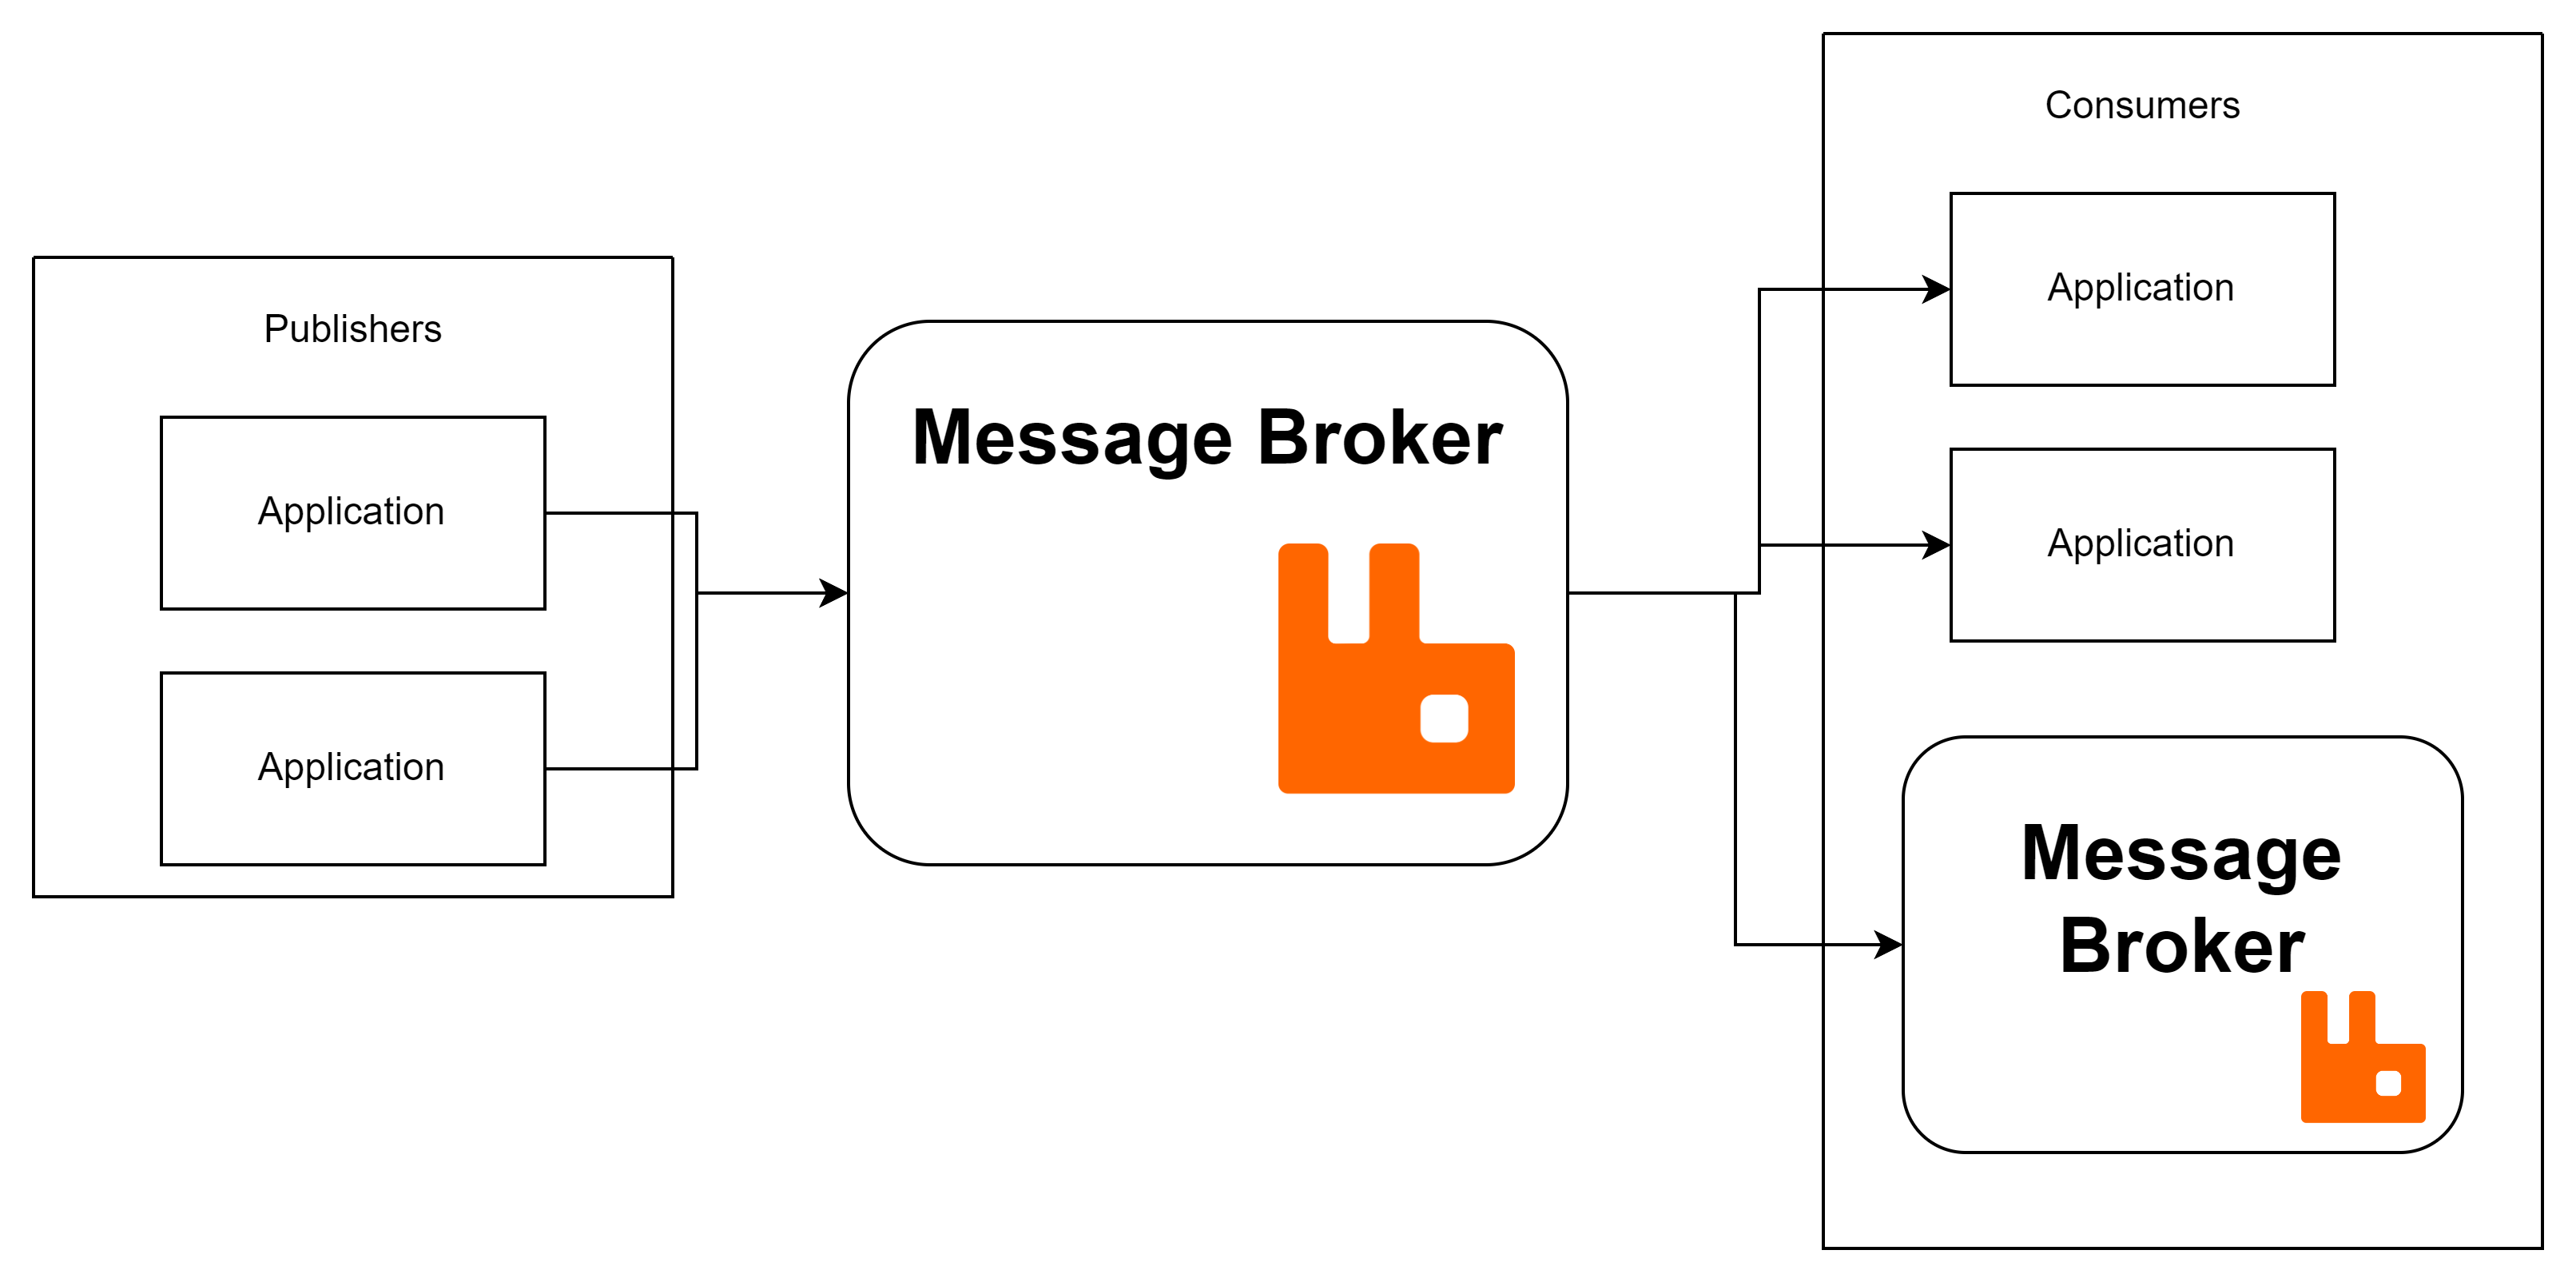
\includegraphics[width=\linewidth]{Service Bus Architecture}
    \caption{Service Bus Architecture}
    \label{fig:serviceBusArchitecture}
    \source{Opracowanie własne}
\end{figure}

\par Przykładami popularnych \emph{Message Broker}ów są: \emph{RabbitMQ}, \emph{Apache Kafka}, \emph{ActiveMQ}, \emph{AWS SNS/SQS} i \emph{Azure Service Bus}.